\chapter{Software de programación y ensayo del control digital}
% ----------------------

\label{C:Software de programación y ensayo del control digital}

\section{Características físicas del microcontrolador}
En esta sección se explorará de manera breve pero sustancial la lógica interna que gobierna el funcionamiento del Arduino Nano y las diversas tareas que este microcontrolador es capaz de realizar. El Arduino Nano, conocido por su versatilidad y eficiencia en proyectos de electrónica y automatización, que al igual que cualquier otro dispositivo programable, requiere un software bien planificado para ejecutar sus funciones de manera óptima.

\subsection{Lógica Interna del Arduino Nano}
El Arduino Nano, como todos los microcontroladores de la familia Arduino, opera mediante la ejecución de un conjunto de instrucciones programadas en su memoria flash. Estas instrucciones, escritas en el lenguaje de programación C/C++ utilizando el entorno de desarrollo integrado (IDE) de Arduino, dictan cómo el microcontrolador debe responder a diferentes señales y entradas. En esta sección, se abordarán los conceptos básicos de esta lógica interna, incluyendo el ciclo de procesamiento del Arduino, la gestión de interrupciones, y la manipulación de puertos y registros.

\subsection{Pinout de arduino nano}
Se presenta a continuación en la Figura \ref{F:arduino_nano} un \textit{pinout} del Arduino Nano indicando la funcionalidad que presenta en cada una de sus conexiones.
\begin{figure}[H]
    \centering
    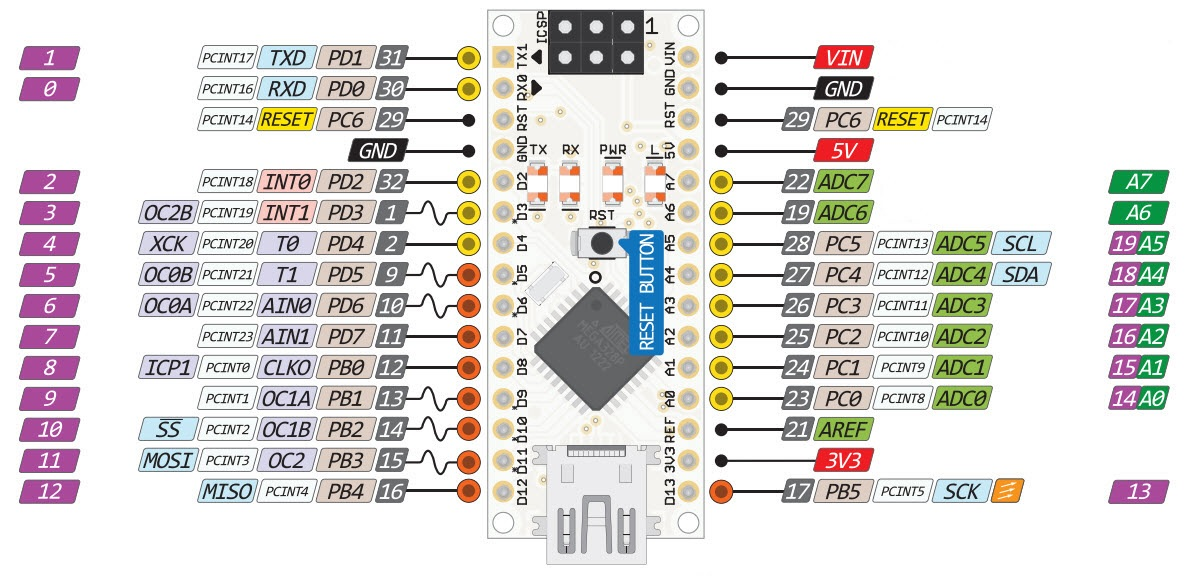
\includegraphics[width=\textwidth]{./imagenes/arduino_nano.jpg}
    \caption{Arduino Nano.}
    \label{F:arduino_nano}
\end{figure}\par 
\underline{Entradas}:
\begin{itemize}
    \item Teclado: 8 pines. 
    \item Sensado de las variables mediante el ADC (SCL; SDA).
\end{itemize}\par 
\underline{Salidas}:
\begin{itemize}
    \item Display. Aislador I2C. DAC.  (SCL; SDA).
    \item Acople Desacople de carga. 1 PIN.
\end{itemize}\par 

\subsection{Protocolo de comunicación.}
El protocolo de comunicación es fundamental en el diseño y desarrollo de sistemas embebidos, ya que define la manera en que los dispositivos intercambian información entre sí. En el caso del Arduino Nano, se cuenta con diversas opciones de protocolos de comunicación, cada uno con sus propias características y aplicaciones específicas. \par 
Entre los protocolos de comunicación compatibles con el Arduino nano se encuentran:
\begin{itemize}
    \item SPI™ (Serial Peripheral Interface): Permite la comunicación síncrona entre dispositivos mediante una línea de reloj común y líneas separadas para datos de entrada y salida.
    \item I2C™ (Inter-Integrated Circuit): Proporciona una interfaz de comunicación de bus de dos cables que permite la comunicación entre múltiples dispositivos conectados al mismo bus.
    \item Universal Asynchronous Receiver Transmitter (UART): Permite la comunicación serial asíncrona entre el microcontrolador y otros dispositivos periféricos.
\end{itemize}\par 
Para este proyecto en particular, se optará por emplear el protocolo I2C debido a su compatibilidad con los componentes utilizados en la fuente disponibles en el mercado Argentino. La elección de este protocolo se fundamenta en su eficiencia y versatilidad, lo que lo hace idóneo para satisfacer los requisitos de comunicación de este sistema embebido.
La forma en que interactuan y se conectan los dispositivos entre sí en base al protocolo se indica en la Figura \ref{F:diagrama_protocolo_i2c}.

\begin{figure}[H]
    \centering
    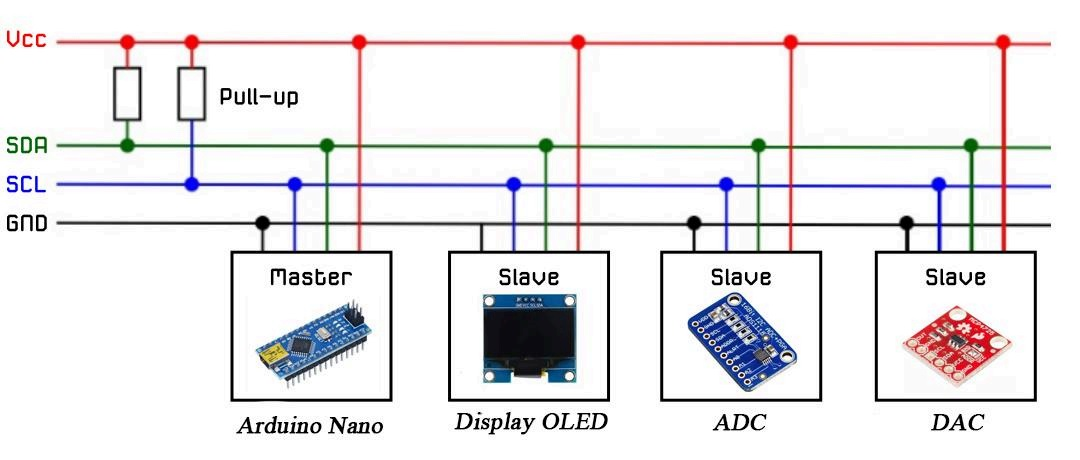
\includegraphics[width=0.8\textwidth]{./imagenes/i2cprotocol.jpg}
    \caption{Conexionado típico de protocolo I2C.}
    \label{F:diagrama_protocolo_i2c}
\end{figure}

Durante la comunicación con los demás dispositivos mediante el canal I2C el Arduino Nano toma el rol de único maestro. Debido a que todos se encuentran conectados en una misma línea la forma de acceder a cada dispositivo independientemente de los demás es mediante el uso de direcciones de 7 bits. En este caso estas serán las que se encuentran a continuación. Sin embargo se recuerda que estas en algunos casos son determinadas por la conexión del pin ADDRESS de los componentes, así que ante cualquier duda debe consultarse la hoja de datos del elemento correspondiente.
\begin{itemize}
    \item ADC ADS1115 ADDRESS: 0x48
    \item DAC MCP4725 ADDRESS: 0x60
    \item Display OLED ADDRESS: 0x3C
    \item Potenciómetro MCP4661 ADDRESS: 0x28
\end{itemize}

\subsection{Dependencias y Librerías Empleadas}

Una de las ventajas más destacadas de trabajar con Arduino es su activa y extensa comunidad, que ha desarrollado una vasta colección de librerías para simplificar la escritura de código y la implementación de funcionalidades avanzadas. Estas librerías permiten a los desarrolladores enfocarse en la lógica central de sus proyectos, sin tener que preocuparse por programar desde cero cada tarea sencilla. A continuación, se presentan las principales librerías utilizadas en este proyecto:

\begin{itemize}
    \item \textbf{Key.h}: Esta librería facilita la gestión de entradas de teclado, permitiendo la detección y el procesamiento eficiente de pulsaciones de teclas.
    \item \textbf{Keypad.h}: Utilizada para manejar teclados matriciales, esta librería simplifica la lectura de teclas y la interpretación de entradas de usuario.
    \item \textbf{Wire.h}: Esencial para la comunicación I2C, esta librería permite la interacción con una variedad de dispositivos periféricos compatibles con este protocolo, como sensores y expansores de E/S.
    \item \textbf{Adafruit\_ADS1X15.h}: Proporciona soporte para la familia de convertidores analógico-digital (ADC) ADS1X15 de Adafruit, permitiendo lecturas precisas de señales analógicas.
    \item \textbf{Adafruit\_GFX.h}: Una librería gráfica que proporciona primitivas de dibujo básicas, tales como líneas, círculos y texto, utilizada comúnmente en pantallas gráficas.
    \item \textbf{Adafruit\_SSD1306.h}: Especializada en el control de pantallas OLED basadas en el controlador SSD1306, esta librería facilita la visualización de información en pantallas compactas y de alta resolución.
    \item \textbf{Adafruit\_MCP4725.h}: Proporciona una interfaz sencilla para controlar el DAC MCP4725, permitiendo la generación de señales analógicas de manera precisa.
\end{itemize}

\section{Ensayos y simulación}
Para los ensayos de los modelos constructivos, se utilizó el software simulador de circuitos electrónicos Proteus 8 Professional. Este software proporciona una serie de herramientas que permiten evaluar el funcionamiento de los componentes implementados en el control digital de manera eficiente. \par 
Una de las características más destacadas de Proteus 8 Professional, y la razón principal por la que se prefiere frente a otras alternativas, es su comunidad activa. Esta comunidad ha desarrollado librerías extensivas de componentes, incluidos microcontroladores Arduino. Estas librerías no solo incluyen las huellas (footprints) de los componentes, sino que también permiten programarlos de manera similar a como se haría con los dispositivos reales. Esta funcionalidad es particularmente valiosa, ya que permite al diseñador observar una simulación precisa de la interacción entre todos los elementos, sirviendo como base para la implementación con componentes físicos en etapas posteriores del desarrollo.

En la Figura \ref{F:esquematico_proteus} se presenta resumidamente la etapa digital del proyecto, indicando la interconexión de los distintos módulos al microcontrolador.
\begin{figure}[H]
    \centering
    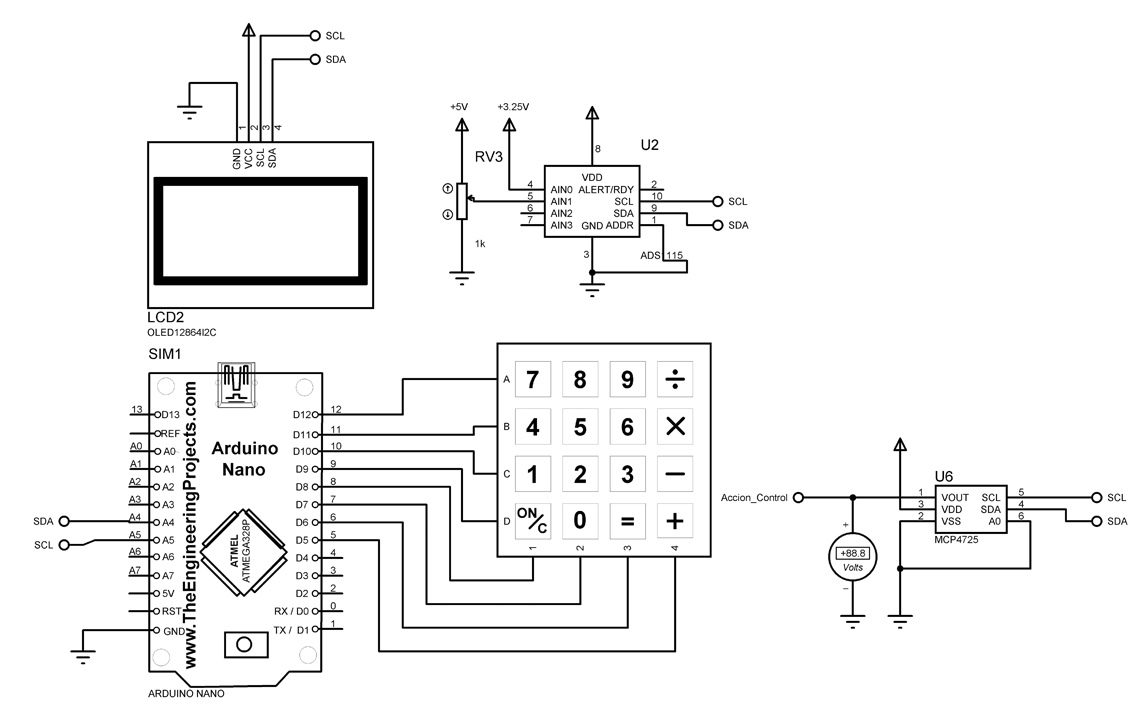
\includegraphics[width=\textwidth]{./imagenes/proteus_esquema2.jpg}
    \caption{Esquemático de conexión de los componentes digitales para un primer ensayo.}
    \label{F:esquematico_proteus}
\end{figure}

\section{Resultados Experimentales}
Basado en el desarrollo descrito en la sección anterior, se obtuvo un modelo funcional de circuito y código que cumplía con los objetivos propuestos del sistema de control. Esto culminó en el ensayo físico de los componentes utilizando una base \textit{protoboard}, donde se comprobó que todos los elementos funcionaron, siguiendo el esquema provisto en la Figura \ref{F:ensayo_digital}. Así, se concluyó exitosamente el ensayo de esta sección, validando el diseño y su implementación práctica.
\begin{figure}[H]
    \centering
    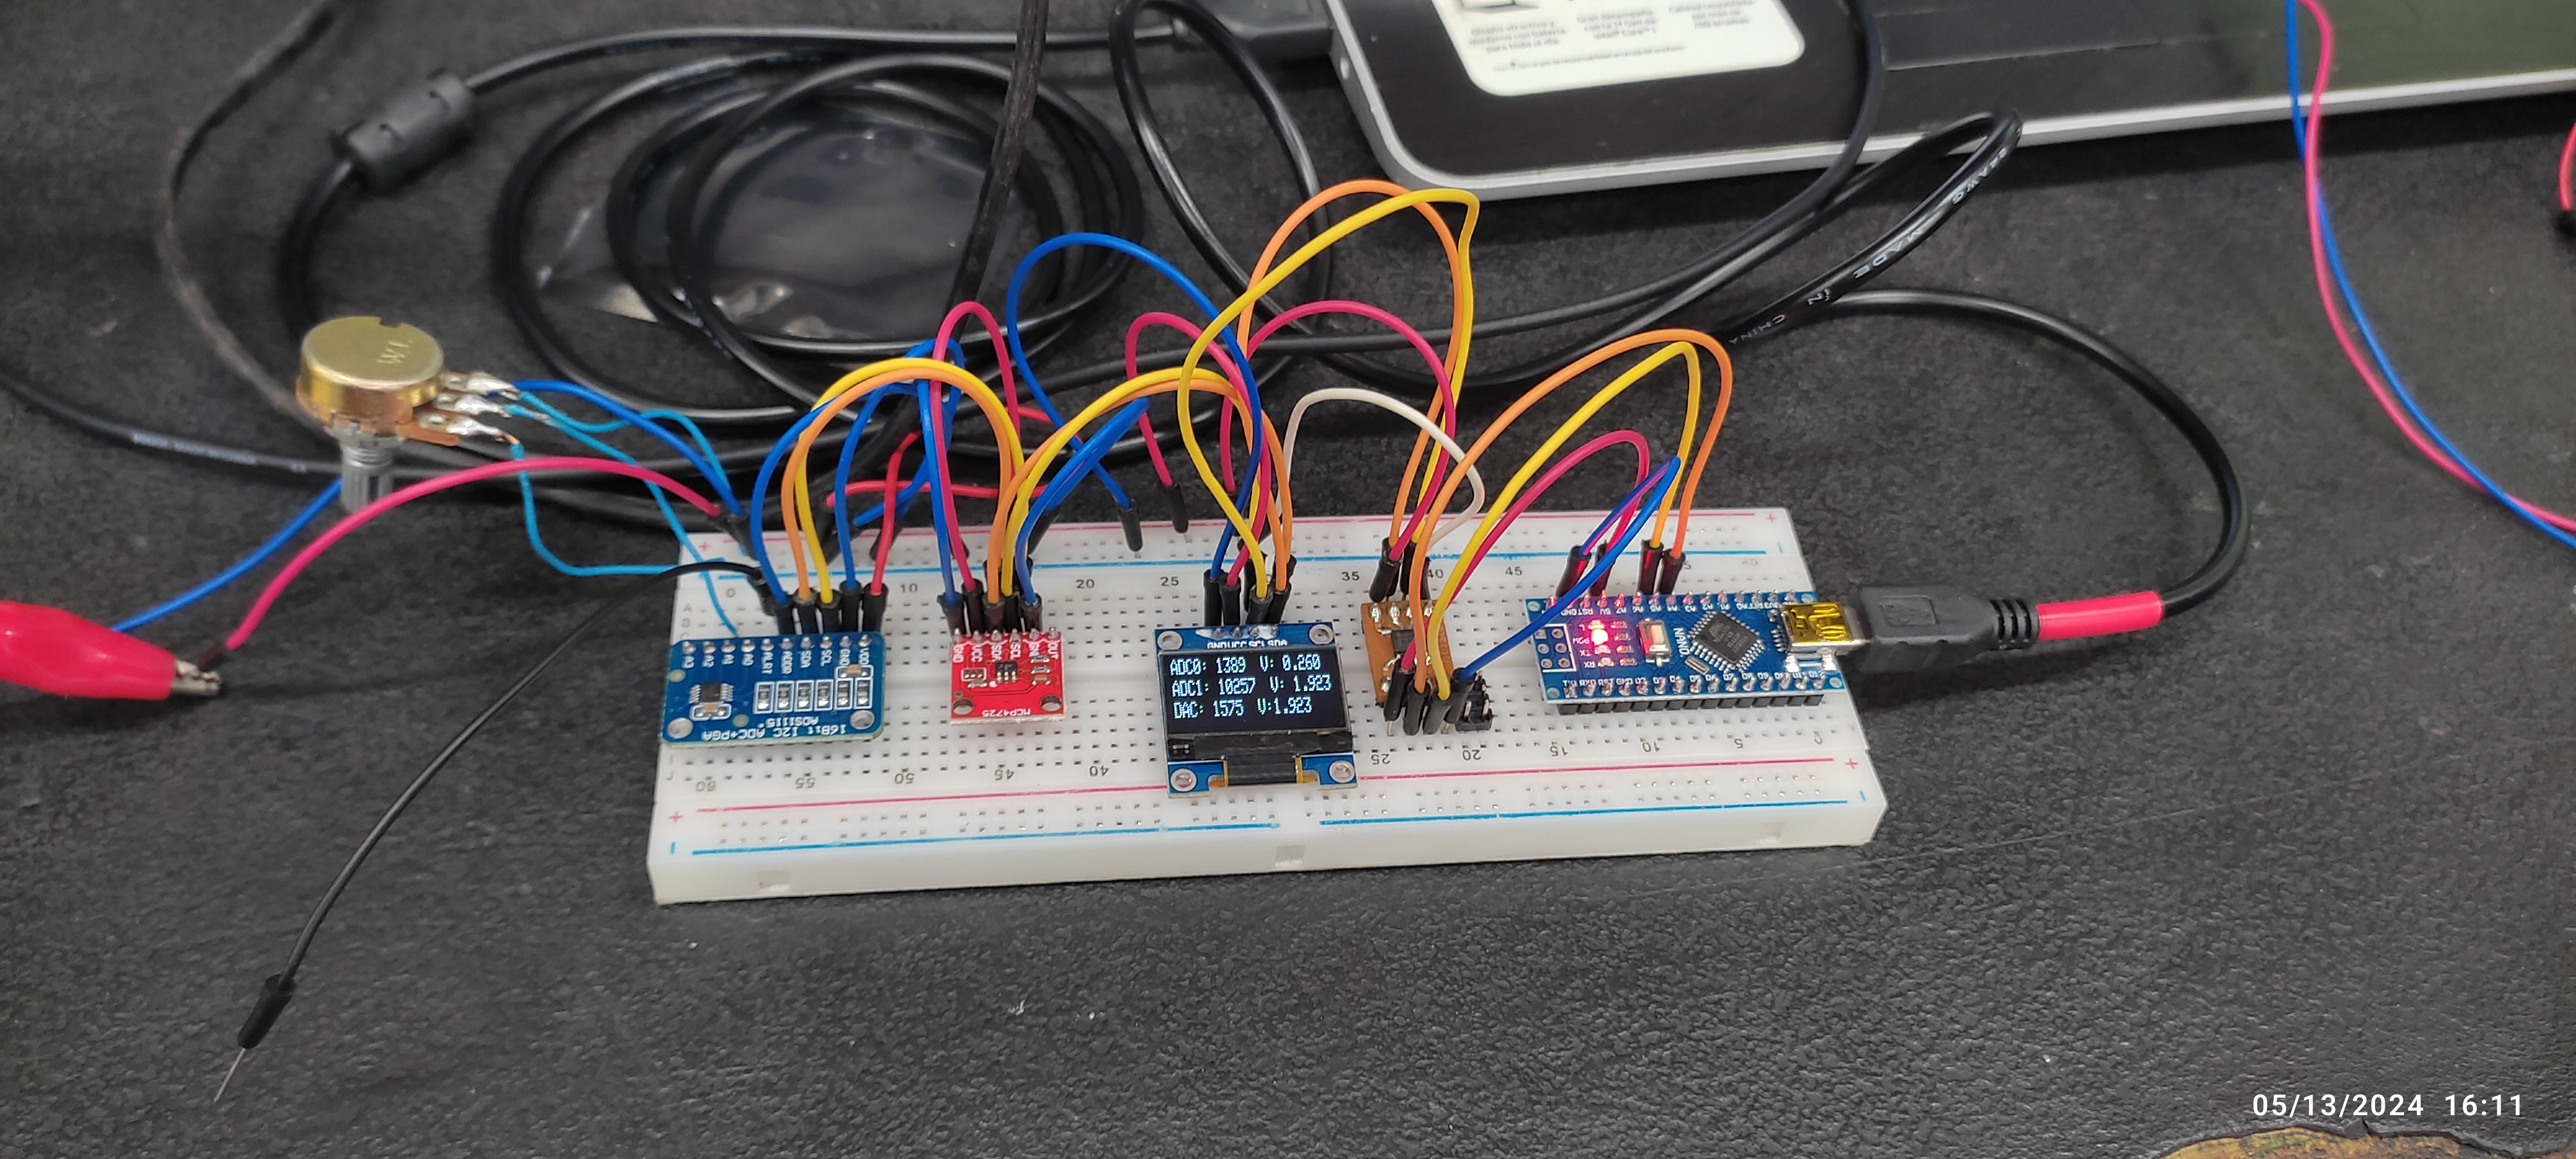
\includegraphics[scale=0.08]{./imagenes/ensayo_digital.jpg}
    \caption{Ensayo en protoboard de los componentes correspondientes a la etapa digital.}
    \label{F:ensayo_digital}
\end{figure}

\section{Diagrama de Control del Software}
El software implementado en el microcontrolador para el control de la fuente de alimentación está diseñado siguiendo una estructura modular y organizada, lo que permite una adecuada secuenciación de las tareas y una toma de decisiones eficiente. El siguiente diagrama de la figura \ref{F:diagrama_de_procesos} muestra el flujo de trabajo del software, representando el orden en el que se ejecutan las distintas funciones y cómo se toman las decisiones dentro del microcontrolador para garantizar un control preciso de la salida.\par
El código del sistema se ha estructurado en cuatro secciones principales, cada una de las cuales cumple una función clave en la operación global:\par
\begin{itemize}
    \item \textbf{Manejo de Presión de Teclas:} Esta sección se encarga de detectar la pulsación de alguna de las teclas del panel de control por parte del usuario. En función de la tecla presionada, se ejecuta la acción correspondiente, como ajustar los valores de referencia de la tensión o corriente de salida, modificar configuraciones, o activar/desactivar la fuente.
    \item \textbf{Manejo de la Interacción con el Encoder:} El encoder rotativo es un dispositivo crucial para la manipulación de las referencias en lazo de control. Esta sección del código capta los movimientos de rotación del encoder, ya sea en sentido horario o antihorario, y actualiza en tiempo real las referencias de tensión y corriente que el sistema debe alcanzar. Gracias a esta implementación, el usuario puede ajustar de manera precisa los valores de salida.
    \item \textbf{Algoritmo de Cálculo de la Acción de Control:} En esta sección se llevan a cabo los cálculos que determinan la acción de control óptima que se enviará al actuador. El algoritmo implementado aplica las ecuaciones correspondientes para calcular las señales de control de corriente y tensión, basándose en los errores detectados entre los valores de referencia y los valores actuales.
    \item \textbf{Actualización del Display:} Esta sección maneja la comunicación con la pantalla de visualización, determinando el momento adecuado para su actualización y los datos que se deben mostrar. Se optimiza para que la pantalla se actualice con una frecuencia controlada, lo que permite al usuario monitorear el estado de la fuente de manera eficiente sin consumir recursos excesivos del sistema.
\end{itemize}

Además de estas secciones principales, se implementaron funciones complementarias, como la \textbf{lectura de datos} y la \textbf{actualización de la Acción de Control}, las cuales se ejecutan con la mayor frecuencia posible para mantener el sistema en funcionamiento estable. También se incluye una rutina de \textbf{asignación de Pines}, que se activa al inicio del programa y determina configuraciones iniciales críticas, como la asignación de direcciones I2C de los dispositivos conectados, la configuración de los pines del relé, y otros parámetros estándares esenciales para la operación de la fuente.

\begin{figure}[H]
    \centering
    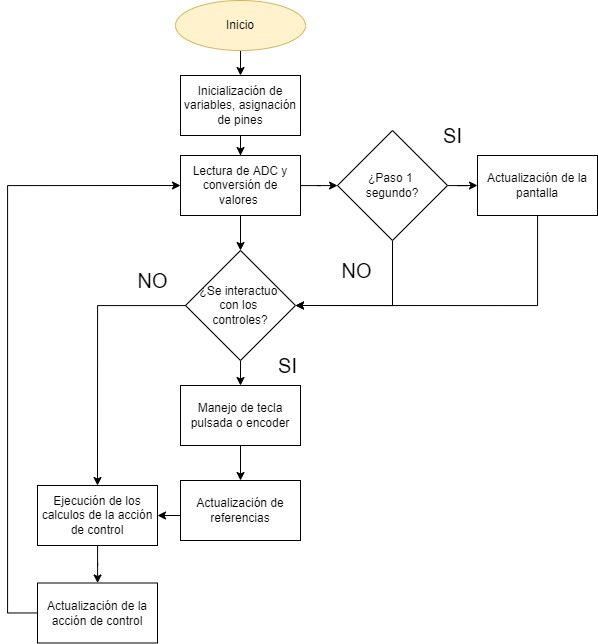
\includegraphics[scale=0.5]{./imagenes/DiagramaDeSoftware.jpg}
    \caption{Diagrama de procesos en el Arduino Nano.}
    \label{F:diagrama_de_procesos}
\end{figure}

\subsection{Detalles y Optimización del Código}
Para lograr un control eficiente y mantener un rendimiento óptimo durante la mayor cantidad de tiempo posible, se realizaron diversas optimizaciones en el código. Estas optimizaciones tienen como objetivo mejorar tanto la velocidad de respuesta del sistema como su estabilidad en condiciones de operación variables. \par
Una de las optimizaciones más relevantes es la decisión de actualizar el display una vez por segundo. Dado que la pantalla no es crítica para el control en tiempo real, esta frecuencia de actualización es suficiente para mantener al usuario informado sin sobrecargar los recursos del microcontrolador. Este ajuste reduce la carga en el sistema, permitiendo que el microcontrolador dedique más tiempo a las tareas críticas, como el cálculo de la acción de control.\par
Otro aspecto importante en el mantenimiento del código fue la \textbf{creación de librerías}. Para mantener un código organizado, accesible y fácil de entender por cualquier usuario o desarrollador, se decidió estructurar el código en C++ mediante librerías dedicadas a cada una de las tareas principales. Esto no solo facilita el mantenimiento del código, sino que también mejora su modularidad, permitiendo la reutilización de secciones de código en futuros proyectos o en modificaciones del sistema. \par
Estas optimizaciones en conjunto contribuyen significativamente al rendimiento general del sistema, asegurando que el control sea robusto y que el software sea fácil de mantener y extender en el futuro.\par
